\chapter{Korištenje cycleGAN arhitekture za semantičku segmentaciju ortopanograma}

\section{Opis problema}

Jedan od najčešće korištenih, pa i najkorisnijih dijagnostičkih alata u području stomatologije su zasigurno rendgenske panoramske snimke čeljusti. Relativno su jednostavne za provođenje, a stomatologu daju velik broj informacija o stanju pacijenta. Međutim, u određenim situacijama, poput prisustva šuma u ortopanogramu, ili većeg broja umjetnih zubi/implanata čak i najboljem stomatologu može biti zahtjevno odrediti točnu poziciju svakog od zuba u čeljusti. Stoga bi programsko rješenje koje bi omogućilo automatsko označavanje svakog zuba u ortopanogramu zasigurno bilo korisno, te bi se, uz primjenu kao pomoćni alat stomatolozima, moglo iskoristiti kao početna točka daljnjim nadogradnjama, poput automatske detekcije bolesti zuba ili slično. Stoga u ovom poglavlju predlažem rješenje za semantičku segmentaciju stomatoloških panoramskih rendgenskih snimaka, temeljnog na cycleGAN arhitekturi.\\

\noindent Kao podatke za treniranje predloženog modela na raspolaganju sam imao dvije vrste ortopanograma: 376 ortopanograma te njihovih pripadajućih segmentacijskih mapa (označenih ručno), te 3950 neoznačenih ortopanograma, odnosno ortopanograma bez pripadajuće segmentacijske mape. Upravo ovakva distribucija podataka, gdje na raspolaganju imamo relativno malen broj označenih slika ali relativno velik broj neoznačenih, je bila glavna motivacija za uvođenje cycleGAN arhitekture. Ta arhitektura bi u teoriji, uz sve označene slike, trebala moći iskoristiti i neoznačene slike prilikom treniranja kako bi poboljšala generalizaciju. 


\begin{figure}%
    \subfloat[Ortopanogram]{{\hspace*{-1cm}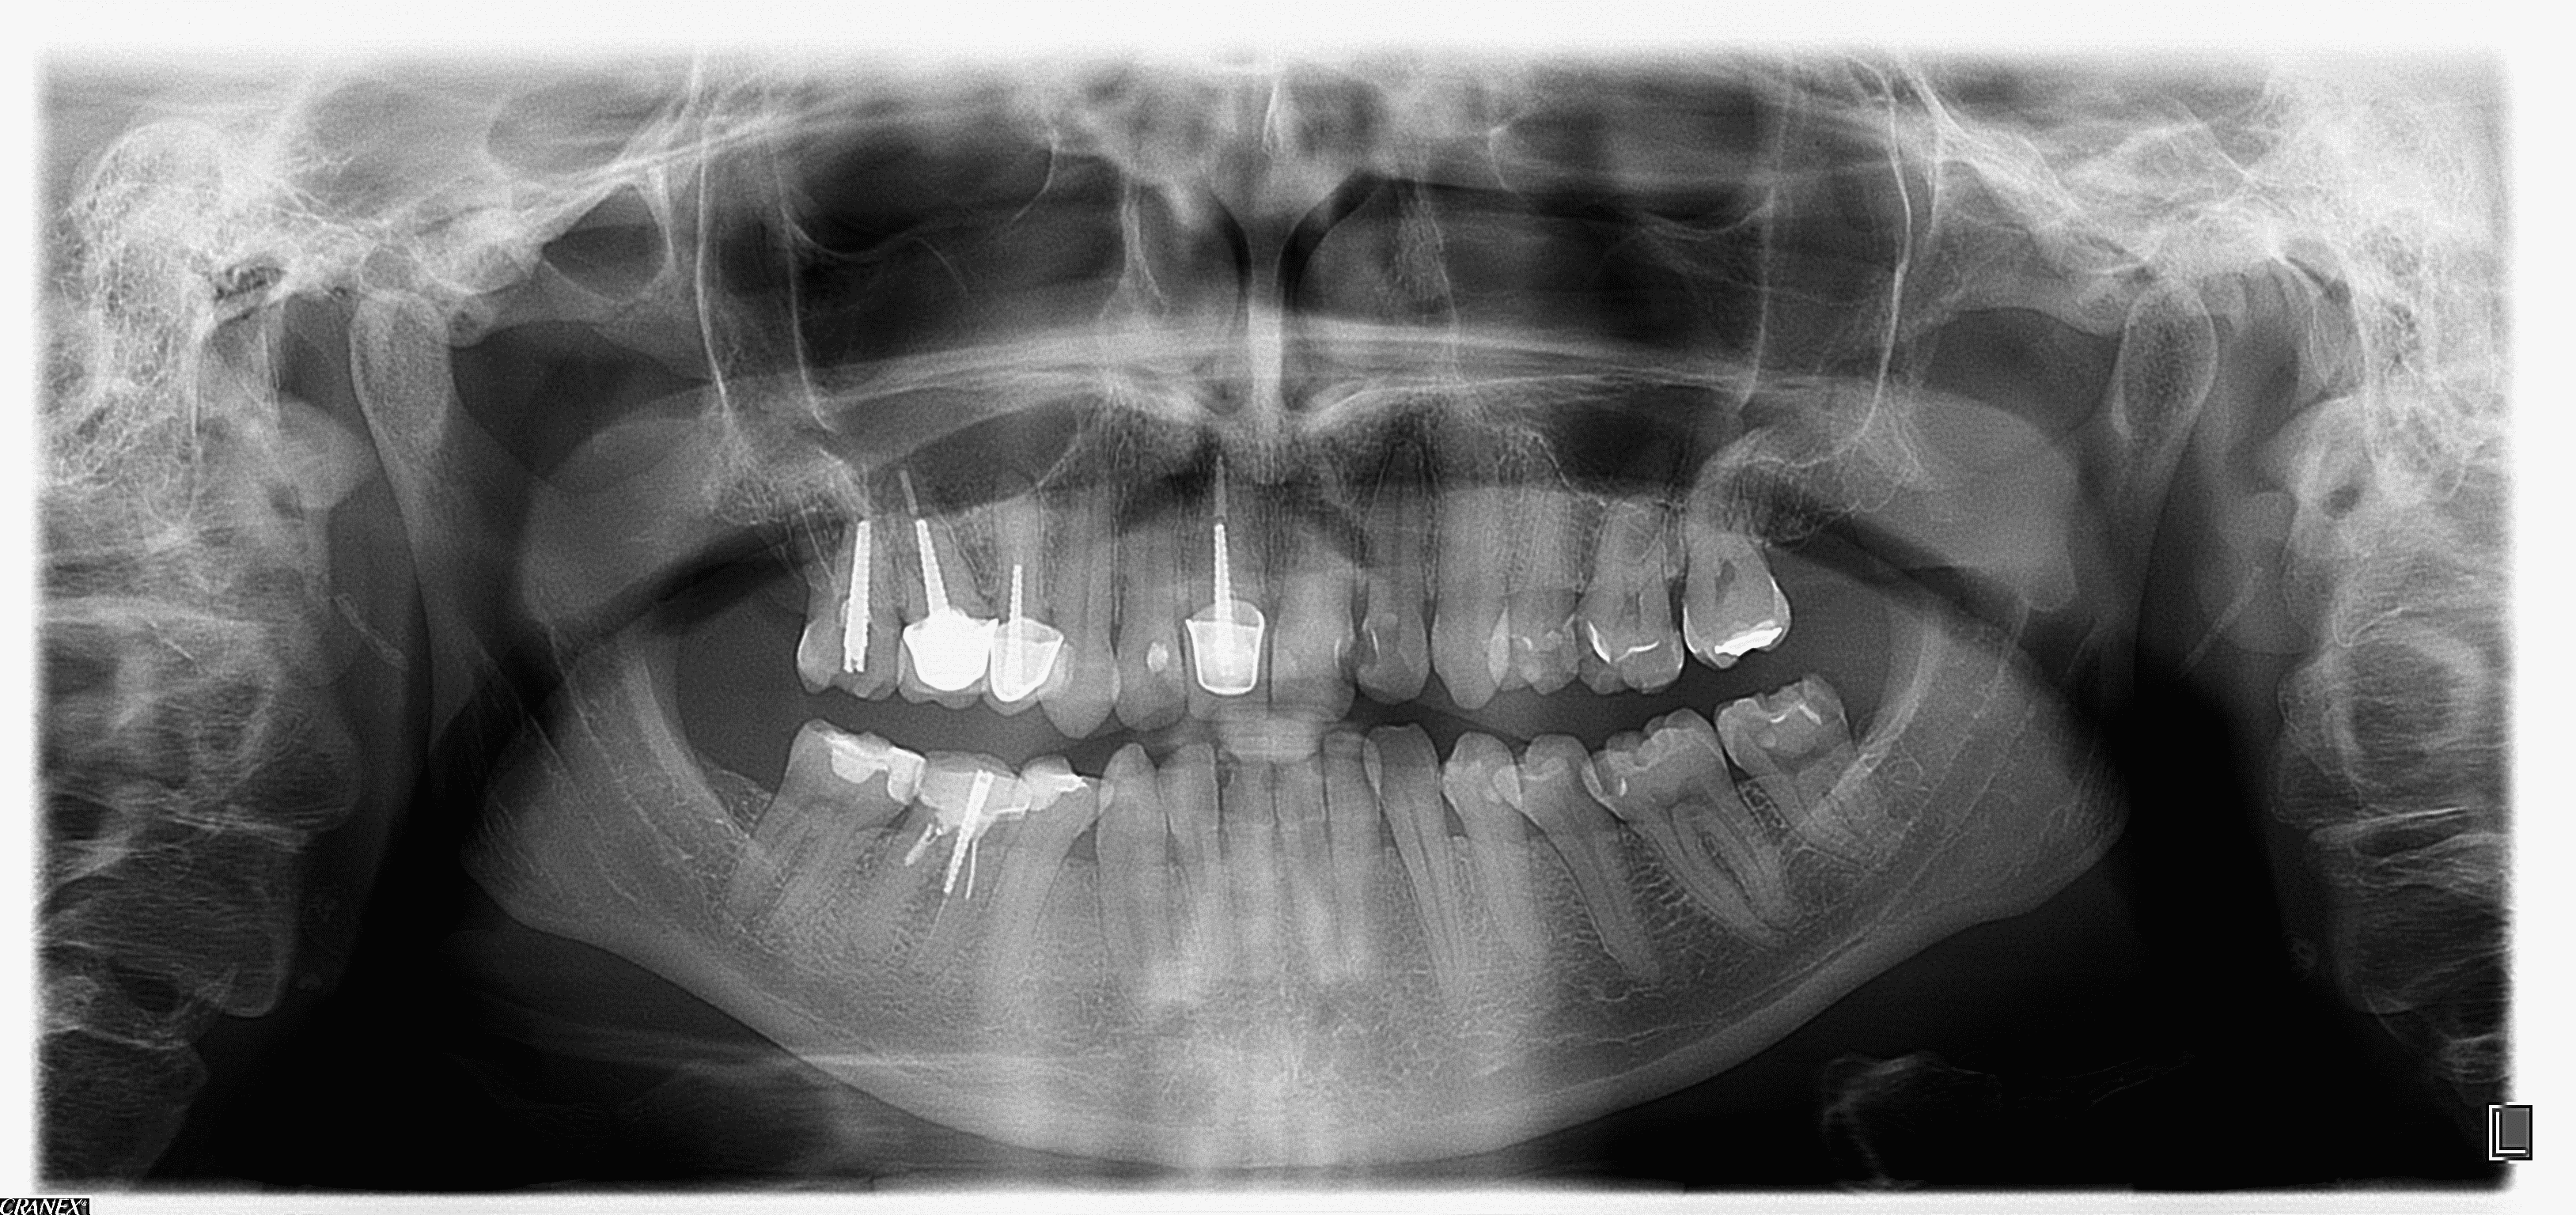
\includegraphics[width=16cm]{slike/ortopanogramPrimjer.png} }}%
    \qquad
    \subfloat[Ortopanogram + segmentacijska mapa]{{\hspace*{-1cm}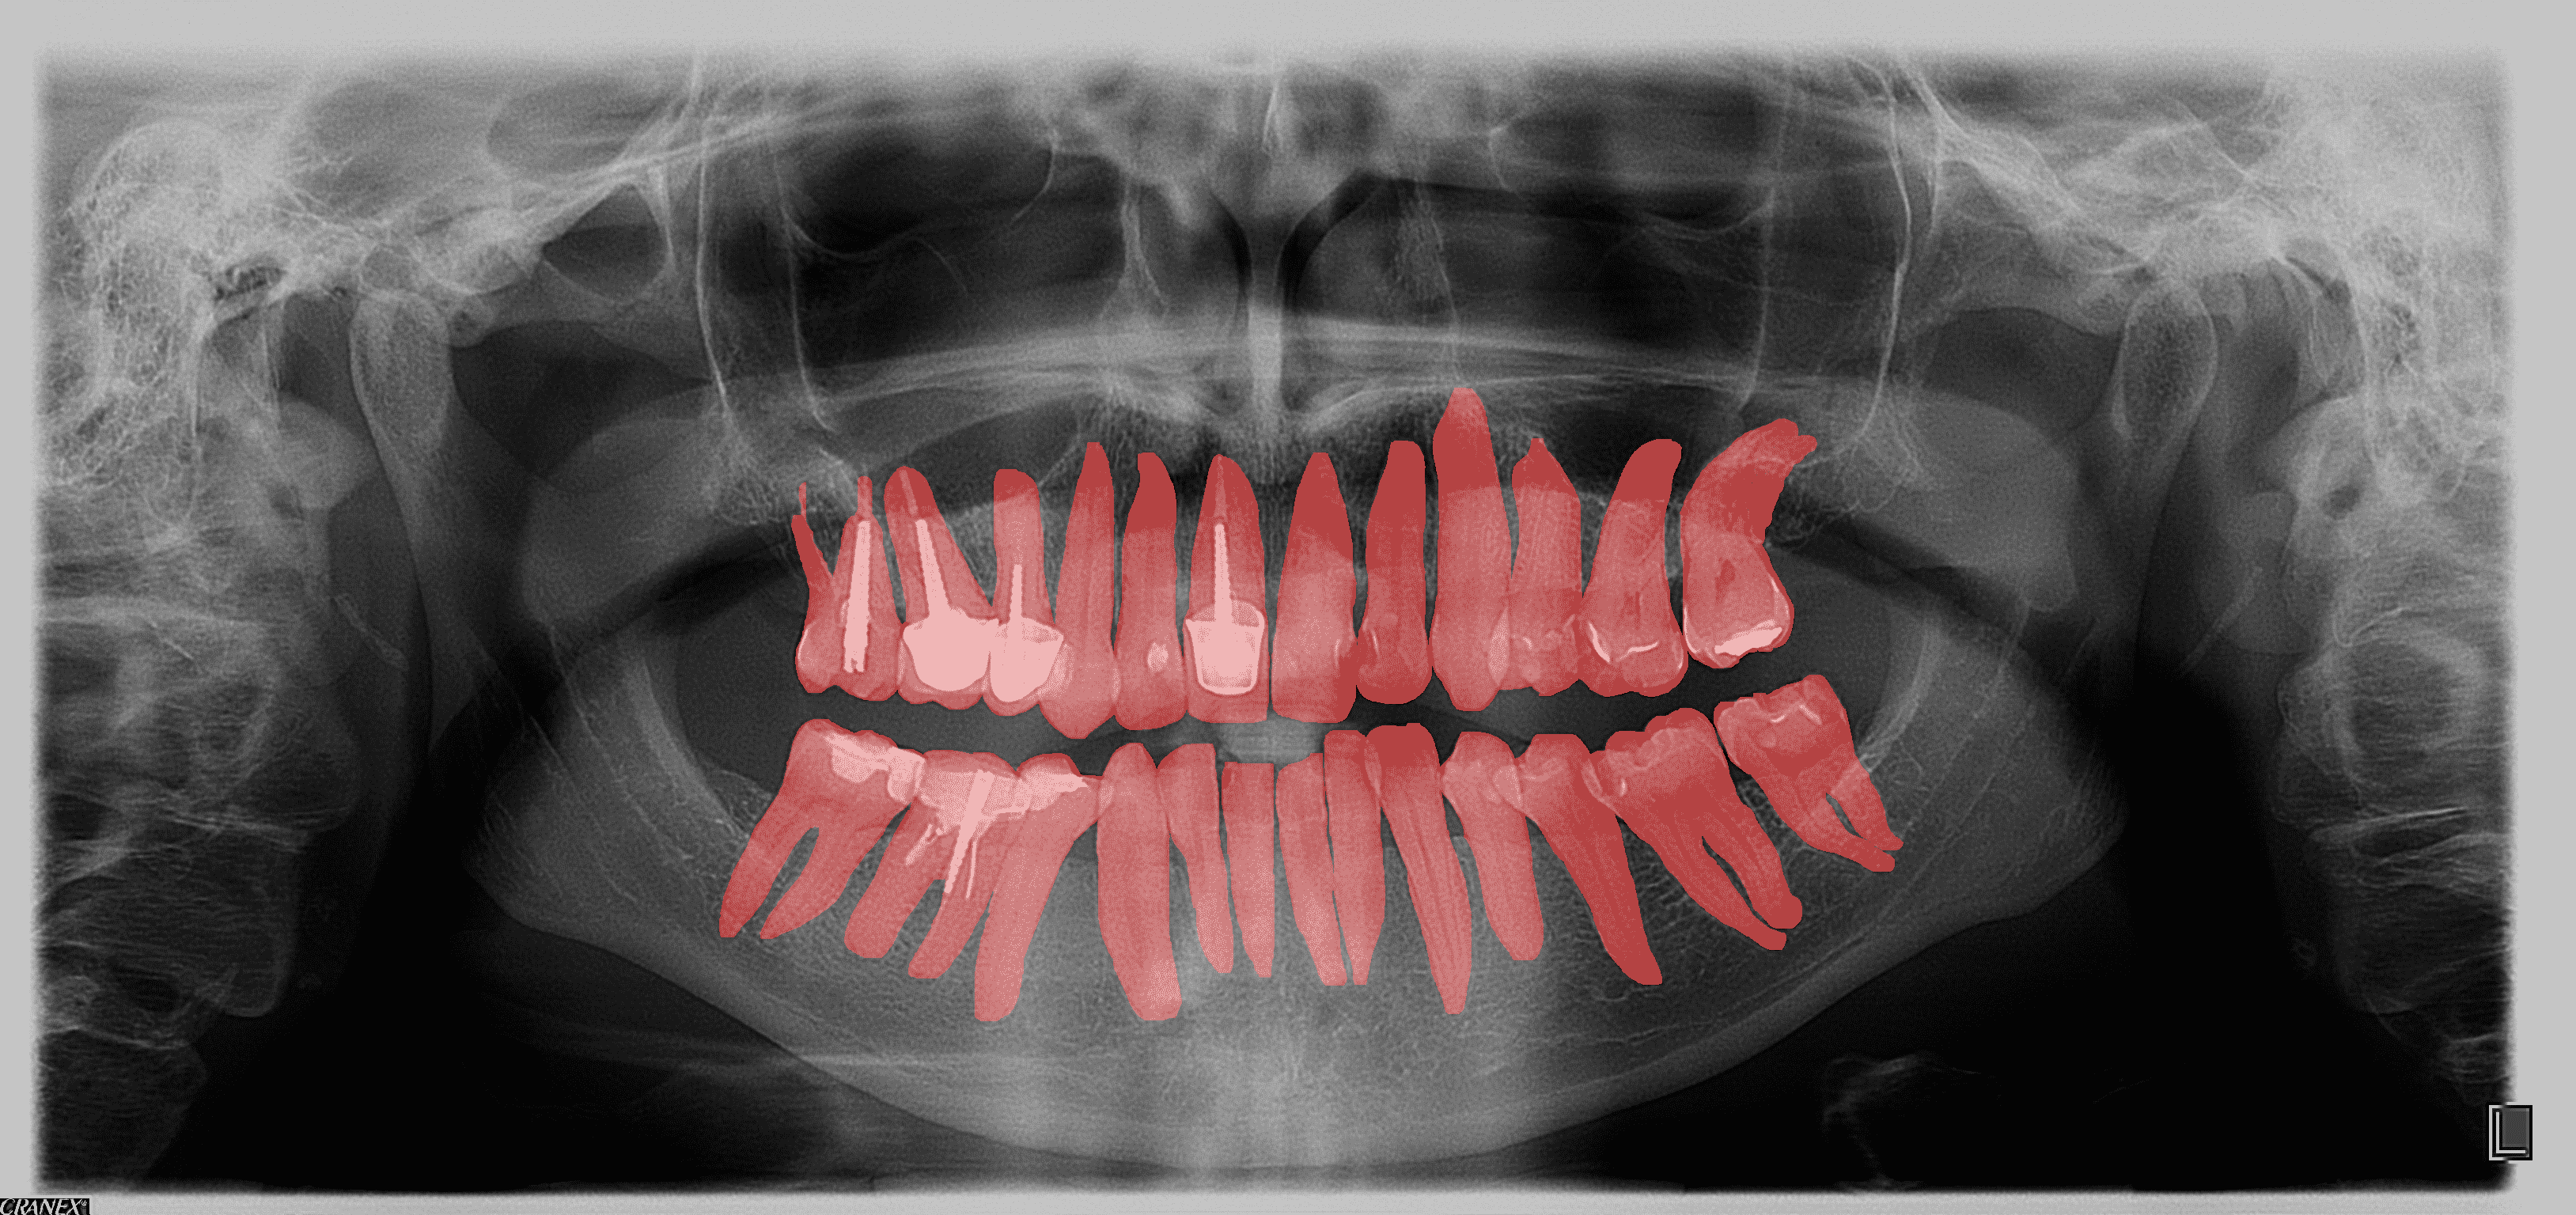
\includegraphics[width=16cm]{slike/ortopanogramPrimjerSegmentacija.png} }}%
    \caption{Ortopanogram i njegova segmentacijska mapa}%
    \label{fig:example}%
\end{figure}



\section{Opis predloženog rješenja}
Korišteno je rješenje prvi put predloženo u \citep{cycleGANSegmentation}. U tom radu autori predlažu iskorištavanje mogućnosti cycleGAN-a za učenje bidirekcijskog mapiranja korištenjem neuparenih slika iz domene A i domene B za polunadziranu semantičku segmentaciju. Navode da korištenjem svojstva cikličke konzistentnosti cycleGAN-a (opisanog u 4.4) model može naučiti bidirekcijsko mapiranje između \textbf{neoznačenih} slika i segmentacijskih mapa. Ovime dodajemo određeni nenadzirani regularizacijski efekt koji poboljšava treniranje, te također imamo način za iskoristiti i neoznačene slike u modelu, do kojih je često puno lakše doći nego do označenih. Baš zato što, uz klasične parove (slika, segmentacijska mapa) koristimo i dodatne neoznačene slike, koje nemaju svoje segmentacijske mape model vrši oblik \textbf{polunadziranog} \engl{semisupervised} učenja. Autori su proveli testiranje predloženog modela na tri skupa podataka (PASCAL VOC 2012, Cityscapes, ACDC), te zaključili da model postiže 2-4\% bolje rezultate u odnosu na odgovarajući potpuno nadzirani model.

U nastavku ću detaljnije opisati arhitekturu korištenog rješenja, kao i modifikacije potrebe za rad s ortopanogramima.
\subsection{Arhitektura rješenja}

Predložena arhitektura rješenja nešto je drugačija od običnog cycleGAN-a. 
Kao i kod običnog cycleGAN modela, predloženi model ima 2 generatora i 2 diskriminatora.Zadaća prvog generatora, kojeg ćemo označiti sa \bm{$G_{IS}$} (od engl. \textit{image to segmentation}), je mapirati slike (ortopanograme) na njihove odgovarajuće segmentacijske mape. Prvi diskriminator, \bm{$D_{S}$}, nastoji razlikovati te generirane segmentacijske mape od originalnih. Drugi generator, \bm{$G_{SI}$} \engl{segmentation to image}, uči kako mapirati segmentacijsku mapu s odgovarajućom slikom tj. ortopanogramom. Ovaj generator se koristi samo za poboljšanje treniranja. Konačno, drugi diskriminator \bm{$D_{I}$} kao ulaz prima sliku ortopanograma te nastoji odrediti radi li se o stvarnoj ili generiranoj slici. Kako bi se osigurala ciklička konzistentnost, generatori se treniraju tako da kad segmentacijsku mapu koju je generirao $G_{IS}$ predamo u $G_{SI}$ kao izlaz dobijemo originalnu sliku ortopanograma. I obrnuto, kad generatoru $G_{IS}$ predamo sliku koju je generirao $G_{SI}$, kao izlaz dobiti originalnu segmentacijsku mapu koju je $G_{SI}$ primio kao ulaz.

No, nije sve tako jednostavno. Uz dodatak opisanim generatorima i diskriminatorima, model ima još dva para generatora, nazovimo ih $\hat{G}_{IS}$, $\hat{G}_{SI}$, te još jedan dodatni diskriminator, $\hat{D}_{I}$. Zanimljivo je da se ovi dodatni generatori i diskriminatori ne spominju u originalnom radu, već su ih autori naknadno dodali u \textbf{službeni} kod modela, priložen radu, uz još nekoliko izmjena. Jedino objašnjenje koje je dano je da se radi o "daljnjim poboljšanjima". Ove 3 mreže se u kodu isključivo koriste na mjestima gdje bi se u običnom cycleGAN-u računala tzv. ciklična pogreška slika. Koriste se na način da diskriminator $\hat{D}_{I}$ odlučuje dolazi li rekonstruirana slika iz ciklusa $\hat{G}_{IS}$, $\hat{G}_{SI}$, ili iz ciklusa 
$G_{IS}$, $G_{SI}$. Iako nisam sasvim siguran zašto su autori odlučili uvesti ove izmjene, u praksi se pokazalo da značajno pridonose uspješnosti modela (mIoU 0.5 za originalni model vs mIoU 0.65 za modificirani model, 33 klase). Iz tog razloga odlučio sam koristiti modificiranu arhitekturu umjesto one predložene u samom radu.\\

\noindent Kako bi formalnije definirali predloženu arhitekturu, kao i korištene funkcije gubitka, uvedimo sljedeću nomenklaturu: sa \bm{$\mathcal{X_{L}}$} označimo skup označenih slika (dakle ortopanograma koji u skupu segmentacijskih maski imaju svoj par), sa \bm{$\mathcal{Y_{L}}$} skup svih originalnih segmentacijskih maski \engl{ground truth}, te sa \bm{$\mathcal{X_{U}}$} skup svih neoznačenih slika ortopanograma (dakle ortopanograma koji nemaju svoj par u skupu segmentacijskih maski). 

Uvodimo prvu funkciju gubitka, \bm{$L^{S}_{gen}$}. Radi se o nadziranoj funkciji pogreške za segmentaciju, čija je zadaća naučiti $G_{IS}$ da, na osnovu predane slike ortopanograma generira odgovarajuću segmentacijsku mapu. Funkciju definiramo kao:

\begin{myequation}%
\bm{L^{S}_{gen}(G_{IS}) = \mathbb{E}_{x,y \sim \mathcal{X_{L}}, \mathcal{Y_{L}}}[\mathcal{H}(y,G_{IS}(x)]}  %
\end{myequation}

\noindent gdje $\mathcal{H}$ predstavlja \textbf{unakrsnu entropiju} \engl{cross-entropy} po pikselima:

\begin{myequation}%
\bm{\mathcal{H}(y,  \hat{y}) =  \sum\limits_{j=1}^N   \sum\limits_{k=1}^K y_{j,k}log\hat{y}_{j,k}  }  %
\end{myequation}

\noindent U danoj jednadžbi za $\mathcal{H}$, $y_{j,k}$ predstavlja vjerojatnosti da piksel $j \; \epsilon \; (1, ..., N)$ originalne segmentacijske mape ima oznaku $k \; \epsilon \; (1, ..., K)$, gdje je K broj oznaka. Kako se radi originalnim oznakama, za $y_{j,k}$ ta vjerojatnost je uvijek 1 ili 0 - piksel ili ima tu oznaku ili nema. 
$\hat{y}_{j,k}$ predstavlja slične vjerojatnosti, samo za generiranu segmentacijsku mapu.\\

\noindent Za $G_{SI}$ koristimo L1 normu kao nadziranu funkciju gubitka, kako bi procijenili razliku između originalne označene slike, te slike koju $G_{SI}$ generira iz njene pripadajuće segmentacijske mape:

\begin{myequation}%
\bm{L^{I}_{gen}(G_{SI}) = \mathbb{E}_{x,y \sim \mathcal{X_{L}}, \mathcal{Y_{L}}}[||G_{SI}(y) - x||_{1}]}  %
\end{myequation}

\noindent Prisjetimo se, L1 norma se računa kao apsolutna razlika između dobivenih i očekivanih vrijednosti.

\noindent Kako bi iskoristili neoznačene ortopanograme, uvodimo još dvije vrste funkcija gubitka: suparničke funkcije gubitka i funkcije gubitka za cikličku konzistentnost.

Ako je $D_{S}(y)$ predviđena vjerojatnost da segmentacijska mapa $y$ odgovara originalnoj segmentacijskoj mapi, suparničku funkciju gubitka za $D_{S}$ možemo definirati kao:

\begin{myequation}%
\bm{L^{S}_{disc}(G_{IS},D_{S}) = \mathbb{E}_{y \sim \mathcal{Y_{L}}}[MSE((D_{S}(y))] +
\mathbb{E}_{x' \sim \mathcal{x_{U}}}[MSE(( D_{s}(G_{IS}(x'))))]
}  %
\end{myequation}

Vidimo da se ustvari radi u funkciji srednje kvadratne greške \engl{mean squared error, MSE}. Funkcija se računa na osnovu uspjeha diskriminatora u razlikovanju pravih i lažnih segmentacijskih mapa. \\

\noindent Funkciju gubitka za drugi diskriminator, $D_{I}$, definiramo na ekvivalentan način:

\begin{myequation}%
\bm{L^{I}_{disc}(G_{SI},D_{S}) = \mathbb{E}_{y \sim \mathcal{Y_{L}}}[MSE(D_{S}(y))] + 
\mathbb{E}_{x' \sim \mathcal{x_{U}}}[MSE(( D_{s}(G_{IS}(x'))]
}  %
\end{myequation}

\noindent Prvu cikličku funkciju gubitka definiramo za segmentacijske mape. Kao što smo rekli, za svaki y (segmentacijsku mapu) očekujemo sljedeće: $G_{IS}(G_{SI}(y))  = y$. Ovakvo ponašanje možemo poticati koristeći sljedeću funkciju gubitka:


\begin{myequation}%
\bm{L_{cycle}^s(G_{IS}, G_{SI}) = \mathbb{E}_{{y \sim y_{\mathcal{L}}}}[\mathcal{H}(y, G_{IS}(G_{SI}(y)))]}  %
\end{myequation}

\noindent Koristimo unakrsnu entropiju jer su labele u segmentacijskim mapama kategorijske varijable. \\

\noindent Pogledajmo još uloge $\hat{G}_{IS}$ ,$\hat{G}_{SI}$ i $\hat{D}_{I}$. Prilikom treniranja generatora, $\hat{D}_{I}$ na ulazu prima rekonstruiranu sliku iz ciklusa $G_{SI}(G_{IS}(\mathcal{X_{U}}))$, te određuje  dolazi li rekonstruirana slika iz ciklusa $G_{SI}(G_{IS}(\mathcal{X_{U}}))$, ili iz ciklusa $\hat{G}_{SI}(\hat{G}_{IS}(\mathcal{X_{U}}))$. Na osnovu te odluke, koristeći MSE, računa se funkcija gubitka za $\hat{D}_{I}$. Tu funkciju gubitka možemo označiti sa $\bm{L_{D_{I}}^1}$.

Tijekom druge faze treniranja, kada treniramo diskriminatore a generatori su fiksirani, računamo funkciju gubitka $L_{D_{I}}^2$, kao:

\begin{myequation}%
\bm{L_{D_{I}}^2 = MSE(\hat{D_{i}}(\hat{G}_{SI}(\hat{G}_{IS}(x))),0) + MSE(\hat{D_{i}}({G}_{SI}({G}_{IS}(x))),1)}  %
\end{myequation}

\noindent Primijetimo, ova funkcija je slična $L_{D_{I}}^1$, samo što u nju ulazi i odluka o rekonstruiranoj slici iz ciklusa  $\hat{G}_{SI}(\hat{G}_{IS}(\mathcal{X_{U}}))$.\\

\noindent Konačno, ukupnu funkciju gubitka možemo napisati kao:

\begin{multline*}
L_{total} = \lambda_{1}L^{S}_{gen}(G_{IS}) + \lambda_{2}L^{I}_{gen}(G_{SI}) + \lambda_{3}L_{cycle}^s(G_{IS}, G_{SI}) -\\ \lambda_{4}L^{S}_{disc}(G_{IS},D_{S}) - \lambda_{5}L^{I}_{disc}(G_{SI},D_{S}) + \lambda_{6}L_{D_{I}}^1 - \lambda_{7}L_{D_{I}}^2
\end{multline*}

\noindent U praksi, treniramo generatore dok su parametri diskriminatora fiksirani, i obrnuto. \\

\noindent Kao što je već rečeno, generatori $G_{IS}$ i $G_{SI}$ zasnivani su na DeeplabV2 arhitekturi, dok su $\hat{G}_{IS}$ i $\hat{G}_{SI}$ zasnivani na ResNet arhitekturi. Korišteni su diskriminatori koji rade na razini piksela, odnosno diskriminator za svaki piksel donosi odluku je li lažan ili ne. Diskriminatori se sastoje od 3 konvolucijska sloja, nakon kojih dolazi \textit{Leaky ReLU} aktivacijska funkcija sa $\alpha = 0.2$.
\noindent Tijekom treniranja također je korišten Adam optimizator s parametrima $\beta_{1} = 0.5$ i $\beta_{2} = 0.999$. Stopa učenja postavljena je na 0.0002, s linearnim padom nakon svakih 100 epoha. U svim eksperimentima veličina grupe \engl{batch} je bila 2. Ukoliko u rezultatima modela nije drugačije navedeno, svi parametri $\lambda$ su jednaki 1.0.\\

\noindent Uz navedeni polunadzirani cycleGAN model, paralelno je treniran i nadzirani model (samo jedan generator, odnosno samostalna DeeplabV2 arhitektura), koji se bavi isključivo segmentacijom ortopanograma (dakle, nema veze s GAN-ovima). On je korišten kao usporedna točka za performanse cycleGAN modela.
\subsection{Programska implementacija}
Za programsku implementaciju korišten je programski jezik Python uz knjižnicu \textbf{\href{https://pytorch.org/}{Pytorch}}, a za praćenje treniranja modela koristan je bio alat \textbf{\href{https://www.tensorflow.org/tensorboard}{Tensorboard}}. Modifikacije koda većinom su uključivale prilagođavanje nove vrste podataka - ortopanograma i njihovih segmentacijskih mapa formatu u kojem ih je model očekivao. U tu svrhu napisan je novi dataloader (naziv za klasu u Pytorchu zaduženu za učitavanje podataka u model) za rad s ortopanogramima. Dodana je funkcionalnost za segmentaciju ortopanograma u 2 klase (pozadina + zubi), 3 klase (gornja zubi, donji zubi, pozadina) te 33 klase (32 zuba + pozadina). Također su bile potrebne manje modifikacije u glavnom dijelu koda, većinom kako bi se podržao rad s novim podacima, te modifikacije dijelova koda zaduženih za testiranje i validaciju. Model je treniran na serveru opremljenom s NVIDIA GeForce RTX 2080 grafičkom karticom, sa 11GB video memorije.
\section{Eksperimentalni rezultati} 

Za evaluaciju dobivenih rezultata korištena je mjera \textbf{srednjeg presjeka nad unijom} \engl{mean intersection over union, mIoU}. Ovo je jedna od najčešće korištenih metoda za evaluaciju segmentacijskih modela. Metoda se zasniva na računanju postotka područja nad kojim se generirana oznaka i stvarna oznaka podudaraju, podijeljeno s unijom njihovih ukupnih područja. U slučaju više od jedne klase, IoU se računa za svaku klasu zasebno, te se na kraju računa prosjek dobivenih veličina. Moguće vrijednosti IoU su [0,1], pri čemu bi vrijednost 1 imao model kod kojeg je svaki piksel generirane segmentacijske mape jednak svakom pikselu originalne segmentacijske mape. mIoU je samo prosječan IoU nad svim uzorcima za validaciju. Formalno, IoU definiramo kao

\begin{figure}[htb]
\centering
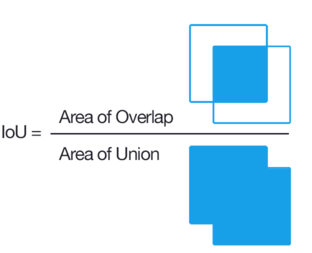
\includegraphics[width=8cm]{slike/miou.png}
\caption{Vizualizacija mIoU-a \citep{miou}}
\label{fig:fer-logo}
\end{figure}
\textbf{}


\noindent Dostupni označeni podaci za treniranje bili su podijeljeni u 3 kategorije: trening (250), validacija (61), testiranje (62). Ako se radilo o nenadziranom (cycleGAN) modelu, tada se u model još i učitavao slučajan podskup od 250 neoznačenih ortopanograma. Trenirani su modeli za segmentaciju 2, 3 i 33 klase. Svaki model je treniran prvo na na 400 epoha, s iznimkom modela s 3 klase, koji je treniran i na 200 epoha. Nakon treniranja tog modela na 200 epoha, zaključeno je da se bolji rezultati dobivaju s 400 epoha, pa su ostali modeli trenirani samo na 400 epoha. Prije ulaska u model, sve slike su postavljene na rezoluciju 200x400, zbog memorijskih ograničenja. Rezultati treniranja modela prikazani su u nastavku.\\

\begin{table}[htb]
\caption{Rezultati modela}
\label{tbl:konstante}
\centering
\begin{tabular}{llr} \hline
Model & Broj epoha & mIoU\\ \hline
Deeplab, 2 klase & 400 & 0.8729981767948044 \\
cycleGAN, 2 klase & 400 & 0.8735012386115315 \\
Deeplab, 3 klase & 200 & 0.8427474738296579 \\
cycleGAN, 3 klase & 200 & 0.8357329101641446 \\
Deeplab, 3 klase & 400 & 0.847020406648659 \\
cycleGAN, 3 klase & 400 & 0.8479922780975828\\
Deeplab, 33 klase & 400 & 0.7023904701665826\\
cycleGAN, 33 klase ($\lambda_{1} = 1.0$) & 400 & 0.650361416818396\\
cycleGAN, 33 klase ($\lambda_{1} = 1.25$) & 400 & 0.6810801346650556\\ \hline
\end{tabular}
\end{table}

\noindent Iz priložene tablice zaključujemo nekoliko stvari. Prva je da se povećanjem broja klasa mIoU smanjuje, no to nije ništa neočekivano. Vidimo da nadzirani (Deeplab) i polunadzirani (cycleGAN) model pri manjem broju klasa postižu gotovo identične rezultate - prilikom treniranja kroz 400 epoha cycleGAN je marginalno bolji, iako razlika je dovoljno mala da ju možemo zanemariti. Također vidimo da, prilikom treniranja sa 3 klase kroz 200 epoha nadzirani model je bio nešto bolji od polunadziranog. Međutim, kad smo broj epoha povećali na 400, polunadzirani model je uspio dostići, pa čak i prestići nadzirani model. Općenito sam primijetio da cycleGAN model sporije konvergira prema minimumu u odnosu na Deeplab model, pogotovo pri početku treniranja, te mogu zaključiti da je cycleGAN bolje trenirati kroz veći broj epoha u odnosu na nadzirane modele. \\ \\

\noindent Rezultati za 33 klase su nešto drugačiji. Vidimo da nadzirani model ima mIoU vrijednost za čak 0.05 bolju od polunadziranog modela, odnosno skoro 8\%. Ovakav rezultat nije u skladu s očekivanjima, jer su autori originalnog rada \citep{cycleGANSegmentation}, dobili bolje rezultate cycleGAN-a u odnosu na nadzirani model u svim slučajevima. Također, radili smo sa relativno malom količinom podataka (250 slika), te je bilo očekivano da će cycleGAN, uvođenjem dodatnih neoznačenih slika poboljšati treniranje. 

Smatram da razlog ovakvoj razlici između nadziranog i polunadziranog modela leži u činjenici da polunadzirani model jednostavno nije (dovoljno) dobro naučio generirati nove slike ortopanograma, što možemo vidjeti iz slika 5.9 te 5.10. Vidimo da je model dobro naučio generirati segmentacijske mape, no da nije bio toliko uspješan prilikom generiranja slika ortopanograma. Slike su mutne i pune šuma, što većinom nije bio slučaj u originalnom radu. Iako te slike jesu u većini slučaja bile dovoljne da bi model iz njih rekonstruirao segmentacijsku mapu ortopanograma, ta mapa se u većini slučajeva ipak djelomično razlikovala od originalne, što je zasigurno negativno utjecalo na treniranje modela. Smatram da je to dijelom zbog relativno malenog skupa podataka, a dijelom i zbog činjenice da su ulazne slike bile niske rezolucije, što odmaže treniranju modela. Također sam primijetio da je funkcija gubitka za diskriminator $D_{I}$ bila vrlo niska (<0.01), što ukazuje na to da je $D_{I}$ vrlo lako zaključivao da se radi o lažnim slikama, što ukazuje na njihovu lošu kvalitetu. Što se tiče funkcija gubitka diskriminatora, pokazivale su slično ponašanje kao i $D_{I}$.
Konačno, kako ukupna funkcija gubitka u cycleGAN modelu ovisi i o funkcijama gubitka zaduženim za generiranje slika, pretpostavljam da su upravo te funkcije gubitka zaustavljale ukupan model da ide prema nižem minimumu. Smatram da je to glavni razlog zašto je nadzirani model postigao bolje rezultate od nenadziranog. 

Djelomično kako bi testirao tu teoriju, a djelomično kako bi poboljšao rezultate modela, trenirao sam još jedan model - cycleGAN sa 33 klase, ali sa parametrom $\lambda_{1}$ povećanim sa 1.0 na 1.25. To je parametar koji određuje koliko funkcija gubitka generatora zaduženog za generiranje segmentacijskih mapa utječe na ukupnu funkciju gubitka. Pretpostavio sam da njegovo povećanje može potaknuti model da se u ukupnoj funkciji gubitka više fokusira na poboljšanje generiranja segmentacijskih mapa, te na taj način smanji utjecaj (loše) generiranih ortopanograma. Dobiveni rezultati potvrđuju tu pretpostavku - mIoU tog modela je za 0.03 uspješniji od mIoU-a istog modela sa $\lambda_{1}$ = 1.0, no i dalje je lošiji od nadziranog modela.\\


\noindent Kao ideju za neka buduća istraživanja, smatram da bi se bilo korisno fokusirati na poboljšanje generiranja neoznačenih slika u modelu, jer se to trenutno čini kao najslabiji dio modela. Korisno bi bilo i mijenjati ostale parametre modela (npr. $\lambda_{2}$, $\lambda_{3}$ itd.) da vidimo kako utječu na model. Također, kao i uvijek prilikom treniranja dubokih modela, rezultati modela bi sigurno bili bolji kada bi na raspolaganju imali više podataka. Bilo bi zanimljivo i pogledati kako rezolucija ulaznih slika utječe na performanse modela - očito je da bi rezultati modela bili bolji, no pitanje je u kojoj mjeri. Trenutno se pokazalo da je za problem segmentacije ortopanograma bolje koristiti neki klasičan konvolucijski model, poput Deeplaba, nego cycleGAN. Osim što se takav model pokazao bolji za segmentaciju većeg broja klasa, pokazuje gotovo identične performanse kao i cycleGAN kod nižeg broja klasa, a pošto puno brže konvergira, može ga se trenirati kroz manji broj epoha nego cycleGAN. Konačno, prilikom treniranja cycleGAN troši skoro 3x veću količinu memorije nego Deeplab (3GB vs 10.5GB), što ga čini prikladnijim i jednostavnijim za treniranje.\\


\noindent U nastavku prilažem slike koje su generirali odgovarajući modeli. U slučaju 2 klase, žutom bojom su označeni zubi, a crnom pozadina. Ako imamo 3 klase, žuto su donji zubi, a crveno gornji. Slično je u slučaju 33 klase, samo što je svaki donji zub označen svojom nijansom žute, a svaki gornji svojom nijansom crvene. \\


\begin{figure}
\begin{tabular}{cccc}
\hspace{-1.5cm}
{
\includegraphics[width = 8cm]{slike/rezultati/supervised2klase1.png}} &
{
\includegraphics[width = 8cm]{slike/rezultati/supervised2klase2.png}}\\
\hspace{-1.5cm}
{
\includegraphics[width = 8cm]{slike/rezultati/supervised2klase3.png}} &
{
\includegraphics[width = 8cm]{slike/rezultati/supervised2klase4.png}}\\
\end{tabular}
\caption{Neki od rezultata nadziranog modela za 2 klase}
\end{figure}

\begin{figure}
\begin{tabular}{cccc}
\hspace{-1.5cm}
{
\includegraphics[width = 8cm]{slike/rezultati/semisuper2klase1.png}} &
{
\includegraphics[width = 8cm]{slike/rezultati/semisuper2klase2.png}}\\
\hspace{-1.5cm}
{
\includegraphics[width = 8cm]{slike/rezultati/semisuper2klase3.png}} &
{
\includegraphics[width = 8cm]{slike/rezultati/semisuper2klase4.png}}\\
\end{tabular}
\caption{Neki od rezultata polunadziranog modela za 2 klase}
\end{figure}

\begin{figure}
\begin{tabular}{cccc}
\hspace{-1.5cm}
{
\includegraphics[width = 8cm]{slike/rezultati/super3klase1.png}} &
{
\includegraphics[width = 8cm]{slike/rezultati/super3klase2.png}}\\
\hspace{-1.5cm}
{
\includegraphics[width = 8cm]{slike/rezultati/super3klase3.png}} &
{
\includegraphics[width = 8cm]{slike/rezultati/super3klase4.png}}\\
\end{tabular}
\caption{Neki od rezultata nadziranog modela za 3 klase}
\end{figure}

\begin{figure}
\begin{tabular}{cccc}
\hspace{-1.5cm}
{
\includegraphics[width = 8cm]{slike/rezultati/semisuper3klase1.png}} &
{
\includegraphics[width = 8cm]{slike/rezultati/semisuper3klase2.png}}\\
\hspace{-1.5cm}
{
\includegraphics[width = 8cm]{slike/rezultati/semisuper3klase3.png}} &
{
\includegraphics[width = 8cm]{slike/rezultati/semisuper3klase4.png}}\\
\end{tabular}
\caption{Neki od rezultata polunadziranog modela za 3 klase}
\end{figure}

\begin{figure}
\begin{tabular}{cccc}
\hspace{-1.5cm}
{
\includegraphics[width = 8cm]{slike/rezultati/super33klase1.png}} &
{
\includegraphics[width = 8cm]{slike/rezultati/super33klase2.png}}\\
\hspace{-1.5cm}
{
\includegraphics[width = 8cm]{slike/rezultati/super33klase3.png}} &
{
\includegraphics[width = 8cm]{slike/rezultati/super33klase4.png}}\\
\end{tabular}
\caption{Neki od rezultata nadziranog modela za 33 klase}
\end{figure}

\begin{figure}
\begin{tabular}{cccc}
\hspace{-1.5cm}
{
\includegraphics[width = 8cm]{slike/rezultati/semisuper33klase1.png}} &
{
\includegraphics[width = 8cm]{slike/rezultati/semisuper33klase2.png}}\\
\hspace{-1.5cm}
{
\includegraphics[width = 8cm]{slike/rezultati/semisuper33klase3.png}} &
{
\includegraphics[width = 8cm]{slike/rezultati/semisuper33klase4.png}}\\
\end{tabular}
\caption{Neki od rezultata polunadziranog modela za 33 klase ($\lambda_{1} = 1.0$)}
\end{figure}

\begin{figure}
\begin{tabular}{cccc}
\hspace{-1.5cm}
\subcaptionbox{}{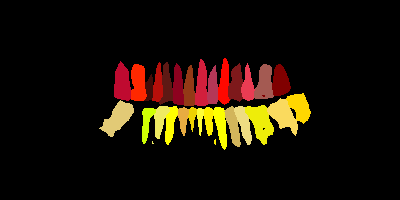
\includegraphics[width = 8cm]{slike/rezultati/train1.png}} &
\subcaptionbox{}{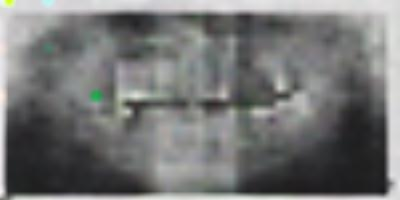
\includegraphics[width = 8cm]{slike/rezultati/train2.jpg}}\\
\hspace{-1.5cm}
\subcaptionbox{}{
\includegraphics[width = 8cm]{slike/rezultati/train3.jpg}} &
\subcaptionbox{}{
\includegraphics[width = 8cm]{slike/rezultati/train4.png}}\\
\end{tabular}
\caption{Prikaz svih generiranih slika tijekom jednog prolaska kroz cycleGAN mrežu, primjer. 1 Slika a) prikazuje prvi prolazak originalne slike kroz $G_{IS}$. Slika b) prikazuje sliku dobivenu prolaskom originalne segmentacijske mape kroz $G_{IS}$, dakle $G_{SI}(x)$. c) prikazuje sliku dobivenu prolaskom generirane segmentacijske mape kroz $G_{SI}$, dakle $G_{SI}(G_{IS}(x))$. d) prikazuje segmentacijsku mapu dobivenu prolaskom b) kroz $G_{IS}$.}
\end{figure}

\begin{figure}
\begin{tabular}{cccc}
\hspace{-1.5cm}
{
\includegraphics[width = 8cm]{slike/rezultati/train2a.png}} &
{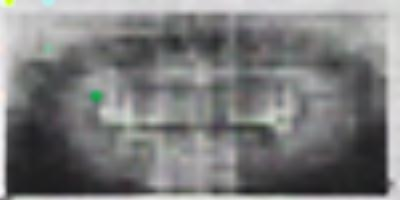
\includegraphics[width = 8cm]{slike/rezultati/train2b.jpg}}\\
\hspace{-1.5cm}
{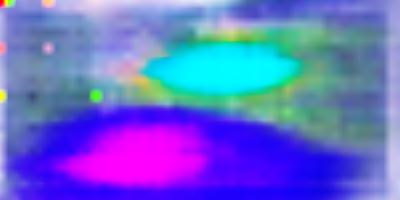
\includegraphics[width = 8cm]{slike/rezultati/train2c.jpg}} &
{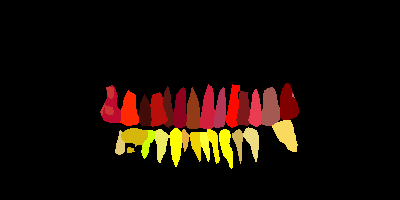
\includegraphics[width = 8cm]{slike/rezultati/train2d.png}}\\
\end{tabular}
\caption{Prikaz svih generiranih slika tijekom jednog prolaska kroz cycleGAN mrežu, primjer 2}
\end{figure}









